\newpage
\section{METHODOLOGY}
In this chapter we will discuss about Data Collection, Data Preprocessing , Metrics used to evaluate the results.

    \subsection{Datasets}
        We use different datasets for training and testing purposes. We tried CelebA dataset, Outdoor Scene Test(OST) datasets and finally landed upon  Common Objects in Context dataset(COCO) for training purposes.
        \begin{figure}[ht]
            \centering
            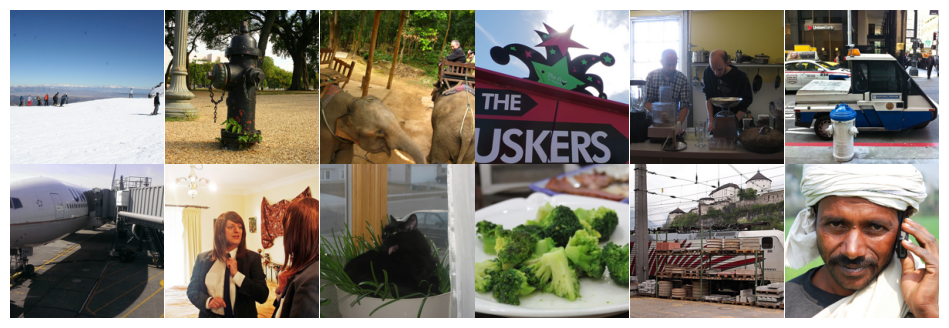
\includegraphics[width=5in]{./figures/train.png}
            \caption{COCO Set Images}
            % \centering
            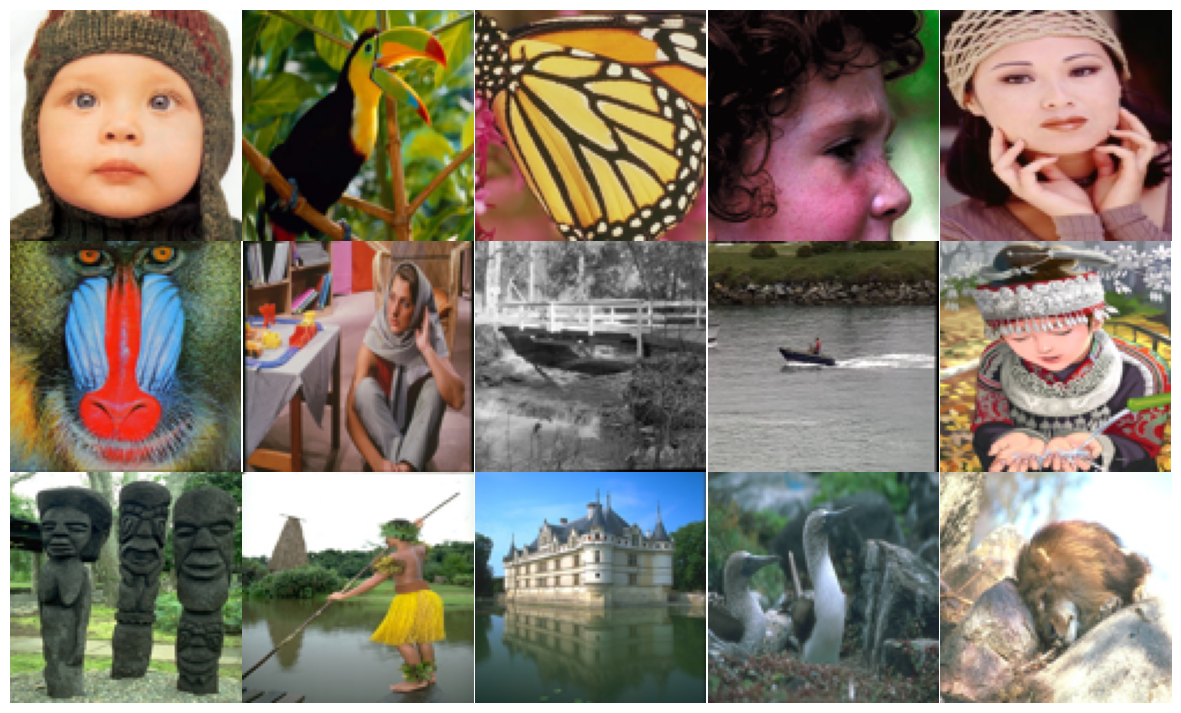
\includegraphics[width=5.5in]{./figures/test.png}
            \caption{Test Set Images(Set5, Set14, BSDS100)}
        \end{figure}  \\
        We are using 2014 variant of COCO dataset. It contains 83k train images and 41k validation images. We are using both of these sets as training set images in our case. We have a total of 124k training images. We have used three famous testing datasets used in Super Resolution application Set5, Set14 and BSD100. They are industry standard testing data sets. We are using to these test datasets to calculate PSNR and SSIM and superesolve them to compare between different superesolved images.
        \subsection{Data Preprocessing}
 We can't process the images directly as images are very resource intensive, We need to train on the cropped patches of images. And to train generator we need high resolution and low resolution version of same patch. In Data Preprocessing step we crop and downsample the images. 
    \begin{itemize}
        \item Cropping: We need to crop a random patch of image every time. So We create a function to give  valid left, top, right, bottom postion of images for a certain patch size. In this case we use 96x96 patch of an image. We then use crop function of the PIL library to crop a patch of image by passing those postions.
        \item Downsampling: We use Bicubic downsampling  to downsample the cropped patch of image by a scaling factor of 4 in this case. Bicubic Downsampling is a method used to reduce the resolution of an image by averaging pixel values in a specific way. It is commonly employed in image processing and computer graphics when it's necessary to create a lower-resolution version of an image.
    \end{itemize}
    \subsection{Training}
    The training process is explained below
    \begin{enumerate}[label=(\roman*)]
        \item For SRCNN:
        \begin{itemize}
            \item Input: Downsampled images of size 24x24 for 4x scaling and 32x32 for 3x scaling only in Y-channel.
            \item Optimizer: Adam optimizer with a learning rate of 1e-4.
            \item Loss function:Mean Squared Error (MSE) loss between the generated images and the original high-resolution images.
        \end{itemize}
        \item For SRResNet:
        \begin{itemize}
            \item Input: Downsampled images of size 24x24.
            \item Optimizer: Adam optimizer with a learning rate of 1e-4.
            \item Loss function:Mean Squared Error (MSE) loss between the generated images and the original high-resolution images.
        \end{itemize}
        \item For SRGAN
        \begin{enumerate}[label=(\alph*)]
            \item Input: Down sampled images of size 24x24.
            \item Optimizer: Adam optimizer with a learning rate of 1e-4.
            \item Loss Function: \\
            Perceptual Loss = Content Loss + Adversarial Loss
            \begin{itemize}
                \item Content loss: MSE loss but computed in the feature space of a VGG19 network. The VGG19 extracts features from both the super-resolved image and the original image, and the MSE is computed on these feature representations.
                \item Adversarial loss: Binary Cross Entropy (BCE) with Logit Loss. The super-resolved images are fed into the discriminator, and the output of the discriminator is used to calculate the adversarial loss.
            \end{itemize}
        \end{enumerate}
    \end{enumerate}
    \subsection{Evaluation Metrics}
    We use PSNR and SSIM as two evaluation metrics to measure the performance of the models. Although, Images perception is very different for humans than these metrics. It provides some theoretical value to compare. The author of SRGAN paper suggested Mean opinion score as a better alternative but it is very difficult to conduct such survey.\\
    \begin{itemize}
        \item {\bf PSNR (Peak Signal-to-Noise Ratio)} is a measure of the quality of a reconstructed or processed image. It compares the peak signal power to the noise power that affects the quality of the image. It can be calculated as :
        \begin{equation}
            PSNR = 10*log_{10}(\frac{MAX^{2}}{MSE})
        \end{equation}
            where MAX is the maximum possible pixel value of the image and MSE (Mean Squared Error) is the average squared difference between the original and the reconstructed images. Higher PSNR values generally indicate better image quality, as it implies lower distortion or noise in the reconstructed image.\\
        \item { \bf SSIM (Structural Similarity Index)} is a metric that measures the structural similarity between two images. It takes into account luminance, contrast, and structure information to provide a more comprehensive assessment of image quality.It can be calculated by using three terms luminance(l), contrast(c) and structure(s) as:
        \begin{equation}
            SSIM(x,y)= \frac{(2*\mu _x*\mu _y+C_1)(2*\sigma_{xy}+C_2)}{(\mu_x^2+\mu_y^2+C_1)(\sigma_x^2+\sigma_y^2+C_2)}
        \end{equation}
        
        where $\mu$ is the mean, $\sigma$ is the standard deviation, and the $\sigma_{xy}$ is the covariance between x and y. $C_1$ and $C_2$ are constants to avoid instability when the denominator is close to zero. \\
        SSIM values range from -1 to 1, where 1 indicates perfect similarity. Higher SSIM values imply better structural similarity between the original and the reconstructed images.
    
    \end{itemize}
    
    